\documentclass[border=10pt]{standalone}
\usepackage{pgfplots}
\pgfplotsset{compat=1.18}

\begin{document}
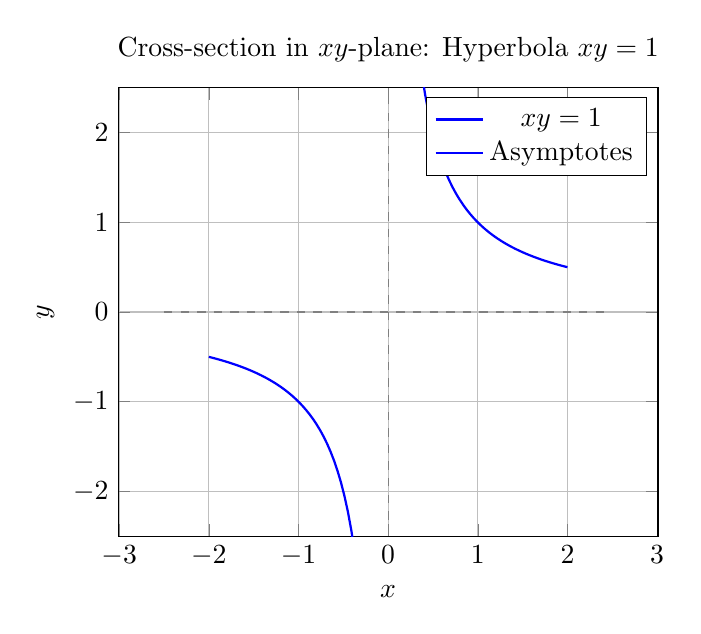
\begin{tikzpicture}
\begin{axis}[
    xlabel={$x$},
    ylabel={$y$},
    title={Cross-section in $xy$-plane: Hyperbola $xy = 1$},
    axis equal,
    grid=major,
    domain=-2.5:2.5,
    samples=100,
    unbounded coords=jump,
    xmin=-2.5, xmax=2.5,
    ymin=-2.5, ymax=2.5,
    ]
    \addplot[blue, thick, domain=-2:-0.1, samples=50] {1/x};
    \addplot[blue, thick, domain=0.1:2, samples=50] {1/x};
    \addplot[dashed, gray, thin] coordinates {(-2.5, 0) (2.5, 0)};
    \addplot[dashed, gray, thin] coordinates {(0, -2.5) (0, 2.5)};
    \legend{$xy = 1$, Asymptotes}
\end{axis}
\end{tikzpicture}
\end{document}